\section{Durchführung}

    In diesem Abschnitt ist die Versuchsdurchführung dargestellt.\\
    Die Abmessungen der verwendeten Kathodenstrahlröhre sind in Abbildung \ref{fig:abmessungen} gegeben.
    \begin{figure}[H]
        \centering
        \includegraphics[angle=270, scale=0.7]{content/img/V501/Abb_5.pdf}
        \caption{Darstellung mit Abmessungen der verwendeten Kathodenstrahlröhre.}
        \label{fig:abmessungen}
    \end{figure}

\subsection{Ablenkung im elektrischen Feld}

    Für diesen Versuch ist eine Kathodenstrahlröhre,
    ein Spannungsgenerator und -messgerät,
    sowie ein Sinusgenerator und ein Frequenzzähler gegeben.\\
   
    Zu Beginn der Messung wird eine Heizspannung an die Kathodenstrahlröhre angeschlossen,
    da diese etwas $\SI{1}{\min}$ vorheizen muss.\\
    \\
    Für die Messung der Verschiebung des Leuchtflecks in Abhängigkeit der Beschleunigungsspannung $U_\text{B}$ ist die folgende Schaltung gegeben.
    \begin{figure}[H]
        \centering
        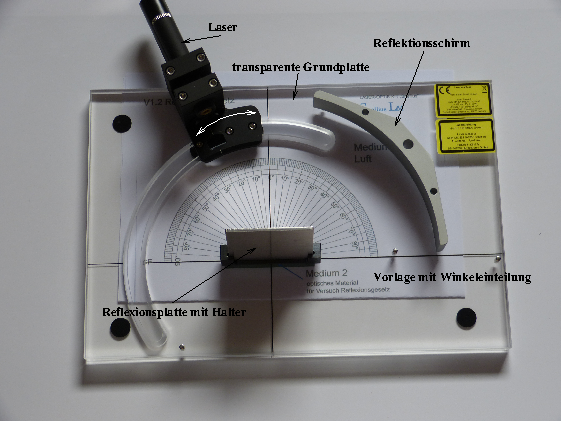
\includegraphics[scale=1]{content/img/V501/Abb_3.pdf}
        \caption{Schaltung einer Kathodenstrahlröhre zur Messung der Proportionalität zwischen Beschleunigungsspannung und Verschiebung.}
        \label{fig:schaltung_kathodenstrahlröhre}
    \end{figure}
    Es muss darauf geachtet werden,
    dass eine der Platten,
    die für die Ablenkung verwendet werden,
    geerdet ist.\\
    Bei der Messung wird nun zuerst die Beschleunigungsspannung $U_\text{B}$ eingestellt.
    Diese liegt in einem Intervall von $U_\text{B} = [\SI{180}{\volt},\SI{500}{\volt}]$.
    Anschließend wird der entstehende Leuchtpunkt auf dem Schirm mithilfe der Spannung $U_\text{C}$,
    welche zur Einstellung der elektrischen Linsen dient,
    fokussiert.
    Danach wird der Punkt so verschoben,
    dass er auf der unteren Linie des Koordinatennetzes auf dem Leuchtschirm liegt.\\
    Nun wird die Ablenkspannung $U_\text{d}$ gemessen,
    indem der Leuchtpunkt immer eine Linie höher geschoben wird und die zugehörige Ablenkspannung von einem Spannungsmessgerät abgelesen wird.\\
    Dies wird für fünf verschiedene Beschleunigungsspannungen aus dem obigen Intervall wiederholt.\\
    \\
    In der nächsten Messung wird die Synchronisationsbedingung in Gleichung \ref{eqn:synchronisationsbedingung} aus Kapitel \ref{sec:oszillograph} untersucht.
    Dazu wird die folgende Schaltung verwendet.
    \begin{figure}[H]
        \centering
        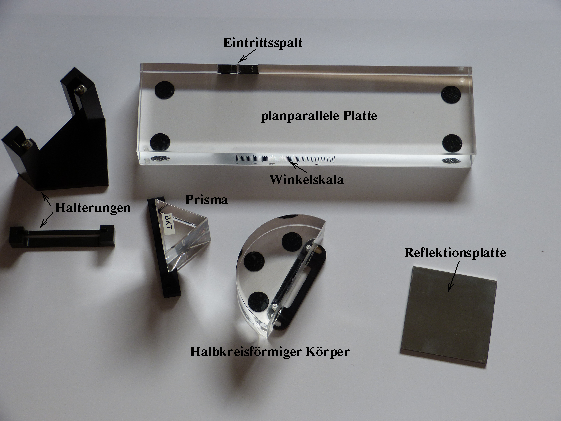
\includegraphics[scale=1]{content/img/V501/Abb_4.pdf}
        \caption{Schaltung eines Kathoden-Oszillographen.}
        \label{fig:schaltung_oszillograph}
    \end{figure}
    Die Beschleunigungsspannung ist bei dieser Messung konstant.\\
    Mithilfe eines Sinusgenerators wird eine sinusförmige Wechselspannung erzeugt,
    und an die Platten der x-Ablenkung wird eine Sägezahnspannung angelegt.
    Diese Spannungen sind immer genau dann Vielfache voneinander,
    wie in Gleichung \ref{eqn:synchronisationsbedingung} vorausgesetzt,
    wenn das Bild auf dem Leuchtschirm zum Stehen kommt.
    Dazu wird mithilfe eines Sägezahngenerators die Frequenz $\nu_\text{Sä}$ variiert,
    bis dies der Fall ist.\\
    Es werden die Werte für $n = \sfrac{1}{2}, 1, 2, 3$ aufgenommen.
    Die Zahl $n$ bezeichnet hier Vielfache der Wellenlänge der Wechselspannung.\\
    Anschließend wird die maximale Ablenkung in y-Richtung,
    also die Amplitude gemessen.

\subsection{Ablenkung im transversalen Magnetfeld}

    Für diesen Versuch ist ein Helmholtzspulenpaar mit Windungszahl $N = 20$ gegeben,
    in dessen Mitte sich eine Kathodenstrahlröhre befindet.
    Die Kathodenstrahlröhre ist an einem Spannungsgenerator angeschlossen,
    während das Magnetfeld der Helmholtzspulen mit einer Stromquelle
    variiert werden kann.
    Zu Beginn der Messungen ist dieses jedoch ausgeschaltet.
    Für die magnetische Flussdichte ist die Gleichung
    \begin{equation}
        B = \mu_0 \frac{8}{\sqrt{125}}\frac{NI}{R}
        \label{eqn:magn_flussdichte}
    \end{equation}
    gegeben mit der Stromstärke $I$ und dem Radius $R$ der Spulen.
    Die Konstante $\mu_0$ beträgt $\SI{4\pi e-7}{\volt \second \per \ampere \meter}$.\\
    \\
    Zu Beginn der Messung wird eine Beschleunigungsspannung aus dem Intervall $U_\text{B} = [\SI{250}{\volt}, \SI{500}{\volt}]$ eingestellt,
    sodass ein Lichtfleck auf dem Leuchtschirm der Kathodenstrahlröhre entsteht.
    Dieser kann mit der Spannung $U_\text{C}$ der elektrischen Linsen fokussiert werden.\\
    Anschließend wird der Lichtpunkt auf die untere Linie des Koordinatennetzes auf dem Leuchtschirm ausgerichtet.
    Um nun die Ablenkung der Elektronen im Magnetfeld zu beobachten,
    wird der Strom an den Helmholtzspulen erhöht,
    sodass der Punkt auf die jeweils nächsthöhere Linie verschoben wird und der entsprechende Stromwert wird auf einem Amperemeter abgelesen.\\
    Dies wird für fünf Beschleunigungsspannungen aus dem obigen Intervall wiederholt.\\
    Die spezielle Ladung der Elektronen kann nun mithilfe der Gleichung \ref{eqn:verschiebung} berechnet werden.
    \\
    In der nächsten Messung soll das Erdmagnetfeld gemessen werden.\\
    Dazu wird zu Beginn der Aufbau mit Helmholtzspulenpaar und Kathodenstrahlröhre so ausgerichtet,
    dass die Strahlachse in Nord-Süd-Richtung zeigt.
    Der Leuchtpunkt wird auf einen Punkt eingestellt und der Aufbau wird in Ost-West-Richtung gedreht,
    sodass sich der Leuchtpunkt auf dem Schirm verschiebt.
    Anschließend wird der Strom in den Helmholtzspulen erhöht,
    sodass das entstehende Magnetfeld die Verschiebung des Erdmagnetfelds kompensiert,
    bis sich der Leuchtpunkt wieder an seiner vorher eingestellten Position befindet.\\
    Zum Schluss muss noch der Inklinationswinkel $\varphi$ zwischen Horizontalebene und der Richtung des Magnetfeldes gemessen werden.
    Dazu wird ein Deklinatorium-Inklinatorium verwendet,
    welches zuerst so ausgerichtet wird,
    dass die Magnetnadel parallel zur horizontalen Drehachse des Aufbaus ausgerichtet ist.
    Danach wird der Teilkreis um $\SI{90}{\degree}$ gedreht und der Winkel abgelesen,
    wobei die Magnetnadel nun in Feldrichtung zeigt.